\documentclass[11pt, letterpaper]{article}
\usepackage{palatino}
\usepackage{graphicx}
\usepackage{enumitem}
\usepackage[top=1in, left=1in, right=1in, bottom=1in]{geometry}
% - - - -  - - - -  - - - -  - - - -  - - - -  - - - -  - - - -  - - - -  - - - -  - - - -  - - - -  - - - -  - - - -  - - - - 
\begin{document}
\begin{center}
\Large{\textbf{Audio Language Classifier:}}

\Large{\textbf{Model Metrics}}

\large{Kirsten Regier}
\end{center}

\section{Gender classifier}
\subsection{Model structure}

Two different models were trained and evaluated for the gender classifier. The structure of each model is shown in Table \ref{tab:GenModels}. 

The models had identical input and output layers. The shape of the input was (32, 10, 128), which corresponds to the batch size (32) and the VGGish embedding (10, 128).  Since the classification was binary, the output layer contained one node, with a sigmoid activation function.

The models differ in the number of hidden layers. Each hidden layer consisted of a dense layer followed by a dropout layer with a dropout rate of 50\%. The first model contained a single hidden layer with 128 nodes. The second model contained two hidden layers, the first with 128 nodes, and the second with 64 nodes. Prior to being fed into the output layer, the output from the previous layer was flattened into a 1D array. The shape of the flattened array varied for each model, based on the number of nodes of the prior layer (128 vs 64).

\begin{table}[!h]
\begin{center}
\caption{Structure of the two gender classifier models. Model 1 has one hidden layer with 128 nodes, while Model 2 has two hidden layers with 128 and 64 nodes, respectively.}
\begin{tabular}{l | c | c |}

Layer  & Model 1 & Model 2\\
\hline

Input 	& (32, 10, 128) & (32, 10, 128) \\ \hline

Dense	& 128 nodes & 128 nodes \\
Dropout	& 50\%		& 50 \% \\ \hline

Dense	&			& 64 nodes \\
Dropout	& 			& 50\% \\ \hline

Flatten 	& (32, 1280)	& (32, 640) \\ \hline
Output 	& (32, 1)		& (32, 1)\\
\hline
\end{tabular}

\label{tab:GenModels}
\end{center}
\end{table}

\subsection{Training time}

Each model was set to run for 100 epochs, or until the validation loss stopped decreasing for 5 consecutive epochs. Model 1 trained for 8 epochs, with the lowest validation loss found at epoch 3. Model 2 trained for 7 epochs, with the lowest validation loss at epoch 2. The evaluation metrics below are based on the weights of the models with the lowest validation loss - after epochs 3 and 2, respectively.

\subsection{Model evaluation}

As shown in Table \ref{tab:GenConfusion}, both models performed quite well on the binary classification task, reaching an accuracy of 98.14\% and 97.55\%, respectively. Model 1 showed similar performance between both classes, with nearly equal numbers of speakers being misclassified from each class. Model 2 showed more discrepancies between the performance of the two classes. Male voices were identified correctly at a rate of 99.14\%, while female voices were identified correctly only 96.5\%. However, the precision of the predictions was the reverse - the precision of female voice prediction was 99.14\%, while the precision of male voice prediction was 96.02\%.

\begin{table}[h]
\begin{center}
\caption{Confusion Matrices for the Gender Classifier Models}
\begin{tabular}{l l | c c r }
\multicolumn{2}{l}{\textbf{Model 1}} & \multicolumn{2}{c}{Predicted} & Recall \\
& & F & M &  \\ 
\cline{2-5}
Actual & F & 590 &  10 & 0.9833 \\
& M & 12 & 572 & 0.9795 \\  \hline
Precision&  & 0.9801 & 0.9828 \\ 
Accuracy & & &  & 0.9814 \\
\end{tabular}
\begin{tabular}{l l | c c r }
\multicolumn{2}{l}{\textbf{Model 2}} & \multicolumn{2}{c}{Predicted} & Recall \\
& & F& M &  \\ 
\cline{2-5}
Actual & F & 576 &  24 & 0.9650 \\
& M & 5 & 579 & 0.9914 \\  \hline
Precision&  & 0.9914 & 0.9602 \\ 
Accuracy & & &  & 0.9755 \\
\end{tabular}
\label{tab:GenConfusion}
\end{center}
\end{table} 

\begin{table}[h]
\begin{center}
\caption{Gender Classifiers - Metrics summary}
\begin{tabular}{l c c}
& 	Model 1 & Model 2 \\ \hline
loss	&0.061640 & 0.076962 \\
accuracy& 0.981419 & 0.975507 \\
precision & 0.982818 & 0.960199 \\
recall & 0.979452 & 0.991438 \\
\end{tabular}
\label{tab:GenMetricsSum}
\end{center}
\end{table} 

Given the slightly better accuracy rates, and the more consistent values of precision and recall between the two classes, it seems that the simpler, one layer model performs slightly better than the more complex, two-layered model for general use cases.

%% Add research about Classifier models - Are male vs female voices harder to classify? Why would we want different rates of precision or recall for the different genders?

% Make up  a story about when to use model one and two based on difference in recall and precision
%- diagnosis vs X
%- minimize false positives
%- use cases for recall (sensitivity) vs precision.

% Screening vs diagnosis
% - screening = find early, non-symptomatic cases in general population
% - diagnosis = find out exactly what is wrong in symptomatic cases

%Model 1 has similar rates of mis-categorizing both male and female voices. About the same number of male voices are identified as female as female voices that are identified as male. Likewise, roughly the same percentage of voices identified as female are actually female and identified as male are actually male. (Roughly equal sensitivity, specificity and precision, roughly equal positive predictive value and negative predicted value).

%Model 2 has higher sensitivity for male voices and lower specificity for female voices. If you expect most of the callers to be male, if the cost is low for misidentifying females as males,

%Model 2 - better sensitivity (recall) for male voices [ but worse specificity for female voices] - identifies male voices as male most of the time; better precision for female voices - fewer predicted female voices were not female. 
%Model 2 has high sensitivity  for male voices, but lower specificity of female voices.  Higher precision for female voices ( more cases predicted female are actually female, fewer cases predicted male are actually male.) More likely to categorize a female voice as male than a male voice as female.
%Model 2 rarely mis-categorizes a male voice as female, but more frequently mis-categorizes a female voice as male. If the model predicts female, the voice is more likely to be female; if the model predicts male, there is slightly less of a chance that the voice is actually male. However, if the voice is actually male, it is more likely that it will be categorized correctly. %If you expect to have mostly male callers, it does a good job identifying them; if you expect mostly female callers, it will have a higher miss rate.

\section{Language classifier}
\subsection{Model structure}

Three models were trained and evaluated for the language classifier. The structure of each model is shown in Table \ref{tab:LangModels}. 

All of the models had identical input and output layers. The shape of the input was (32, 10, 128), which corresponds to the batch size (32) and the VGGish embedding (10, 128).  There were 11 possible classes, so the output layer consisted of 11 nodes. A softmax activation function was used on the output layer, so that the output vector contained the probability that the speaker belonged to each of the output classes. The class with the highest probability was take to the be predicted class.

The models differ in the number of nodes and the number of hidden layers. Each hidden layer consisted of a dense layer followed by a dropout layer with a dropout rate of 50\%. The first model contained a single hidden layer with 12 nodes, while the second model had a single layer with 128 nodes. The third model contained two hidden layers, the first with 128 nodes, and the second with 64 nodes. Prior to being fed into the output layer, the output from the previous layer was flattened into a 1D array. The shape of the flattened array varied for each model, based on the number of nodes of the prior layer (12 vs 128 vs 64).

\begin{table}[!h]
\begin{center}
\caption{Structure of the language classifier models. Model 1 has one hidden layer with 12 nodes, Model 2 has one hidden layer with 128 nodes, and Model 3 has two hidden layers with 128 and 64 nodes, respectively.}
\begin{tabular}{l | c |c  | c |}

Layer  & Model 1 & Model 2 & Model 3\\
\hline

Input 	& (32, 10, 128)& (32, 10, 128) & (32, 10, 128) \\ \hline

Dense	& 12 nodes 	& 128 nodes 	& 128 nodes \\
Dropout	& 50\%		& 50\%		& 50 \% \\ \hline

Dense	&			&			& 64 nodes \\
Dropout	&			& 			& 50\% \\ \hline

Flatten 	& (32, 120)	& (32, 1280)	& (32, 640) \\ \hline
Output 	& (32, 11)		& (32, 11)		& (32, 11)\\
\hline
\end{tabular}

\label{tab:LangModels}
\end{center}
\end{table}

\subsection{Training time}

Each model was set to run for 100 epochs, or until the validation loss stopped decreasing for 5 consecutive epochs. Model 1 trained for 19 epochs with lowest validation loss at epoch 15, %and a final accuracy on the test dataset of 23.30\%.
Model 2 trained for 8 epochs, with the lowest validation loss at epoch 3, and %a final accuracy of 23.86\%.
Model 3 trained for 11 epochs with the lowest validation loss at epoch 6.%, and final accuracy of 25.00\%.
The metrics below are based on the final trained models, with weights from the last trained epoch. % (not from the "best" models)

\subsection{Model evaluation}

The dataset contained many more speakers of English, Spanish and Arabic than speakers of other languages. To balance the classes for the Language Classifier, the number of speakers for these languages was downsampled to 75, which meant that each of these language classes contained 12.0773\% of the total number of speakers in the dataset. German had the fewest number of speakers (36), which comprised 5.797\% of the data. The distribution of the number of \textbf{speakers} sampled per language class is shown in blue in Figure \ref{fig:LangDistTot}. The speakers of each language were split into training, validation and testing sets, so the distribution of speakers in each data split reflects the overall distribution of speakers.  %, as shown in the left panel of Figure \ref{fig:LangDist}.

\begin{figure}[h]
\begin{center}
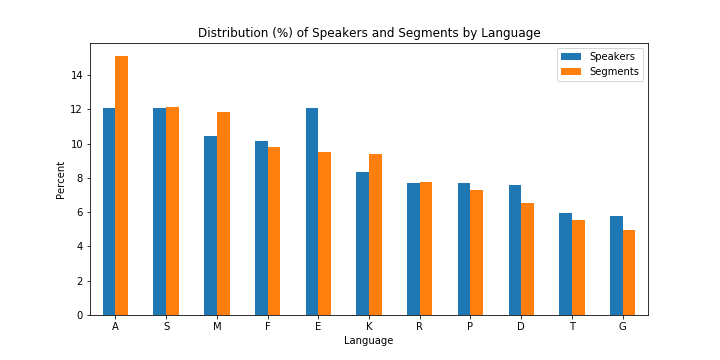
\includegraphics[width=4in]{LangDistPercentSpSeg.png}
\caption{Distribution of Speakers and Segments by Language}
\label{fig:LangDistTot}
\end{center}
\end{figure}

After the speakers were assigned to the data splits, the audio files for all speakers were segmented, and the segments in the training and validation splits were augmented with noise. Since the number of segments per speaker was dependent on the length of the original audio file, which was not determined before the speakers were split, the number of segments per language and per data split were not identical to the distribution of the speakers. 

While the distribution of speakers and segments for most of the languages remains similar (seen by comparing the heights of the blue and orange bars in Figure \ref{fig:LangDistTot}), the distribution of Arabic and English segments changed dramatically. While there were equal numbers of Arabic and English speakers (75 per language, or 12.07\% each), there were 380 Arabic segments and 239 English segments. Thus, the distribution of Arabic segments grew to 15.109344\% of the segments, while the distribution of the English segments shrank to 9.502982\% of segments, moving English behind Spanish, Mandarin and French in the percentage of distribution of the segments.

%\begin{figure}[h]
%\begin{center}
%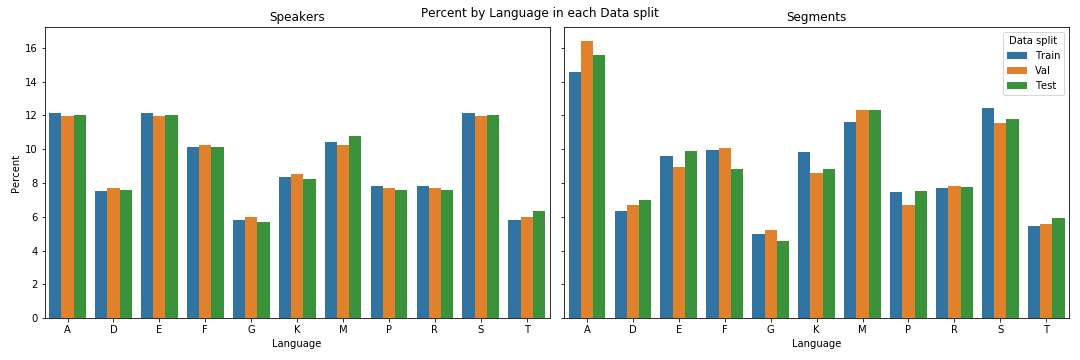
\includegraphics[width=6in]{Lang_PctSpSegLangbySplit.png}
%\caption{Distribution of Speakers and Segments by Language}
%\label{fig:LangDist}
%\end{center}
%\end{figure}

\subsection{Model Metrics}
A naive classifier that always predicted the majority class (Arabic) would have an accuracy of 15\%.  All three of the models improved upon this baseline accuracy rate, as shown in the second row of Table \ref{tab:LangMetricsSum}. While Model 1 has the highest precision rate, it has the lowest accuracy, recall and F1 scores. Model 2 has the highest recall and F1 scores, but also the lowest precision. The most complicated model, Model 3, has the highest overall accuracy, and has F1 scores only slightly lower than Model 2.

\begin{table}[h]
\begin{center}
\caption{Language Classifiers - Metrics summary}
\begin{tabular}{l c c c}
		&Language 1	&Language 2	&Language 3 \\ \hline
Loss		&2.25485		&2.323		&2.20684 \\
Accuracy	&0.232955	&0.238636	&0.25\\
Precision	&0.625		&0.5			&0.605263\\
Recall	&0.0142045	&0.0738636	&0.0653 \\ 

F1 Macro	&0.16999		&0.195512	&0.191103\\
F1 Weighted	&0.20067	&0.228178	&0.224565\\
\end{tabular}
\label{tab:LangMetricsSum} 
\end{center}
\end{table} 

The confusion matrix for the Model 3 predictions is shown in Table \ref{tab:LangConfMat}, with the precision and recall rates by class in Table \ref{tab:LangClassReport}. Not surprisingly, the class with the highest number of correct predictions was the majority class, Arabic, with 24/55 segments correctly predicted (recall of 0.43.63\%) and 24/52 predictions being correct (precision of 0.46.15\%). Dutch, Spanish, English, and Mandarin had 12-15 correct predictions per class. German, the smallest class, along with Russian and Portuguese, had no correct predictions, while Turkish has a single correct prediction.

Behind Arabic, Spanish and Mandarin contributed about the same number of segments to each of the training sets (12.167\% and11.84 \%, respectively). Interestingly, the model made 63 predictions for Spanish and 62 predictions  for Mandarin, which is more than it predicted the majority class. However, since there were fewer correct predictions for Mandarin (15) and Spanish (12), the precision rates for these classes is roughly half that of Arabic.

While Dutch contributed only 6.520875\% of the segments overall, almost half of its testing files were correctly predicted (12/25), making it the class with the highest recall (48\%).

\begin{table}
\begin{center}
\caption{Confusion matrix for Model 3 predictions. The bold numbers on the diagonal represent correct predictions.}
\begin{tabular}{l | c c c c c c c c c c c || c}
lang			&R &A &T &K &G &D &S &F &E &P &M & Segments\\ \hline
Russian		&\textbf{0}  &2  &1  &4  &0  &1  &7  &4  &1  &1  &7 &28\\
Arabic		&0 &\textbf{24}  &0  &4  &1  &7  &2  &2  &4  &0 &11 &55\\
Turkish		&0  &1  &\textbf{1}  &4  &0  &3  &4  &0   &2  &1  &5 &21\\
Korean		&1 &10  &0  &\textbf{6}  &0  &3  &2  &2  &4  &2  &1 &31\\
German		&0  &0  &0  &1  &\textbf{0}  &0  &5  &1  &5  &2  &1 &15\\
Dutch		&0  &4  &0  &0  &0 &\textbf{12} & 3  &1  &3  &1  &1 &25\\
Spanish		&1  &2  &0  &6  &2  &1 &\textbf{12}  &3  &8  &0  &7 &42\\
French		&1  &3  &0  &4  &1  &2 &10 & \textbf{5}  &1  &1  &4 &32\\
English		&0  &1  &0  &3  &0  &5  &2  &2 &\textbf{13}  &0  &4 &30\\
Portuguese	&0  &3  &0  &3  &1  &0  &7  &5  &3  &\textbf{0}  &6 &28\\
Mandarin		&0  &2 & 0  &8  &2  &4  &9  &1  &2  &2 &\textbf{15} &45\\ \hline
Total			&3 &52 &2 &43 &7 &38 &63 &26 &46 &10 &62 &\textbf{352}\\

\end{tabular}
\label{tab:LangConfMat}
\end{center}
\end{table}

\begin{table}
\begin{center}
\caption{Model 3 Metrics by Language}
\begin{tabular}{l c c c| c}
Language  &Precision &Recall &F1-score&Samples\\ \hline
Russian	&0.00	&0.00	&0.00	&28\\
Arabic	&0.46	&0.44	&0.45	&55\\     
Turkish	&0.50	&0.05	&0.09	&21\\      
Korean	&0.14	&0.19 	&0.16	&31\\      
German	&0.00	&0.00	& 0.00 	&15\\       
Dutch	&0.32	&0.48	&0.38	&25\\   
Spanish	&0.19	&0.29	&0.23	&42\\      
French	&0.19	&0.16	&0.17	&32\\    
English	&0.28	&0.43	&0.34	&30\\  
Portuguese&0.00	&0.00	&0.00	&28\\    
Mandarin	&0.24	&0.33	&0.28	&45\\ \hline
      
accuracy		&		&		&0.25	&352\\
macro avg		& 0.21	&0.22	&0.19	&352\\
weighted avg	& 0.23	&0.25	&0.22	&352\\ \hline
\end{tabular}
\label{tab:LangClassReport}
\end{center}
\end{table}

\subsection{Comments}
One question about the language classifier was whether it would identify similarities between languages with historical similarities. For example, Spanish, French and Portuguese are all descendants of Latin, and are more closely related to each other than to other languages in this database, so it would not be surprising for them to be confused with each other more often than with other, unrelated languages.  However, the language classifier showed only weak connections between some related languages.

For example, Portuguese samples were misclassified as French 5 times and Spanish 7 times, but were identified as Mandarin 6 times, and misclassified as Arabic, Korean and English 3 times each. French samples were misclassified as Spanish 10 times, but was more likely to be classified as Korean and Mandarin (4 times each) than Portuguese (1). Spanish samples were only misclassified as French 3 times, but as Mandarin 7 times and Korean 6 times, even though Mandarin and Korean are not related to Spanish. Of the samples that were misclassified as Spanish, 10 were actually French and 7 were Portuguese, but 9 were Mandarin and 7 were Russian. So, while there are weak patterns of misclassification between the Romance languages, Mandarin and Korean also show similar levels of misclassification with Spanish, French and Portuguese.

%Other "common" confusions:
%Korean as Arabic - 10
%French as Spanish - 10
%Arabic as Dutch - 10
%Arabic as Mandarin - 11

%Russian as Spanish and Mandarin, 7 each;  none correct
%Turkish as Mandarin 5
%German  as Spanish and English, 5 each
%Spanish as Korean 6, English 8, Mandarin 7
%Port as Spanish 7, French 5; Mandarin 6
%Mandarin as Korean 8, Spanish 9

%Germanic
%English vs Dutch - 3 D as E, 5 E as D
%Eng vs German - 0 E as G, 5 G as E
%Dutch vs German - 0 D as G, 0 G as D

\end{document}
% - - - -  - - - -  - - - -  - - - -  - - - -  - - - -  - - - -  - - - -  - - - -  - - - -  - - - -  - - - -  - - - -  - - - - 
Groupby language, sum
Sorted in descending order by \% segments

L	Language	Seg	Sp	\%_sp		\%_seg		\%_sp_data	\%_seg_data
A	Arabic	380	75	12.077295	15.109344	36.129857	46.537869
S	Spanish	306	75	12.077295	12.166998	36.129857	35.816711
M	Mandarin	298	65	10.466989	11.848907		31.420528	36.227442
F	French	247	63	10.144928	9.821074		30.498599	28.884452
E	English	239	75	12.077295	9.502982		36.129857	28.463836
K	Korean	237	52	8.373591		9.423459		25.156360	27.267382
R	Russian	195	48	7.729469		7.753479		23.090713	23.331666
P	Portugues	184	48	7.729469		7.316103		23.090713	21.695100
D	Dutch	164	47	7.568438		6.520875		22.801695	20.038110
T	Turkish	140	37	5.958132		5.566600		18.092367	16.974590
G	German	125	36	5.797101		4.970179		17.459455	14.762841

\begin{table}
\begin{center}
\caption{Confusion matrix for Model 2 predictions.}
\begin{tabular}{l | c c c c c c c c c c c || c}
lang			&R &A &T &K &G &D &S &F &E &P &M & Segments\\ \hline

Russian	 &1	&2	&2	&0	&3	&0	&4	&4	&1	&3	&8	& \\
Arabic	&0	& 26	&  0	&  0	&  2	&  6	&  4	&  0	&  3	&  1	& 13	& \\
Turkish	&1	&  2	&  2	&  2	&  1	&  4	&  4	&  1	&  1	&  1	&  2	&\\
Korean	& 5	&  4 	& 2	&  4	&  0	&  3	&  4	&  1	&  1	&  3	&  4	& \\
German	&1	&  0	&  0	&  0	&  0	&  1	&  3	&  2	&  4	&  3	&  1	& \\
Dutch	&1	&  1	& 1	&  0	&  1	& 12	&  1	&  1	&  3	 & 2	&  2	& \\
Spanish	&3	&  1	&  3	&  0	&  4	&  2	&  6	&  2	& 10	&  2	&  9	& \\
French	& 2	&  4	&  1	&  2	&  1	&  1	&  9	&  3	&  3	&  2	&  4	& \\
English	& 1	&  1	&  0	&  1	&  0	&  3	 & 2	&  0	& 15	&  0	&  7	& \\
Portugue	& 7	&  3	&  1	&  3	&  1	&  1	&  1	&  2	&  4	&  1	&  4	& \\
Mandarin	& 1	&  0	&  3	&  5	&  1	&  5	&  9	&  3	&  3	&  1	& 14	& \\  \hline
Total		&23	& 44 & 15 &17 & 14 & 38  & 47 & 19 & 48 & 19 & 68 & 352 \\
\end{tabular}
\label{tab:LangConfMatMod2}
\end{center}
\end{table}

\begin{table}
\begin{center}
\caption{Metrics (precision, recall and F1 score) by language class - Model 3}
\begin{tabular}{l c c c| c c c| c}
& \multicolumn{3}{c}{Model 2} & \multicolumn{3}{c}{Model 3} & \\
Language  &precision &recall	&f1-score	&precision &recall &f1-score&support \\ \hline
Russian	&0.04	&0.04      	&0.04	&0.00	&0.00	&0.00	&28\\
Arabic	&0.59	&0.47      	&0.53	&0.46	&0.44	&0.45	&55\\     
Turkish	&0.13	&0.10      	&0.11	&0.50	&0.05	&0.09	&21\\      
Korean	&0.24	&0.13      	&0.17	&0.14	&0.19 	&0.16	&31\\      
German	&0.00	&0.00	&0.00	&0.00	&0.00	& 0.00 	&15\\       
Dutch	&0.32     	&0.48      	&0.38	&0.32	&0.48	&0.38	&25\\   
Spanish	&0.13     	&0.14      	&0.13	&0.19	&0.29	&0.23	&42\\      
French	&0.16      	&0.09      	&0.12	&0.19	&0.16	&0.17	&32\\    
English	&0.31      	&0.50      	&0.38	&0.28	&0.43	&0.34	&30\\  
Portuguese&0.05      &0.04      	&0.04	&0.00	&0.00	&0.00	&28\\    
Mandarin	&0.21	&0.31      	&0.25	&0.24	&0.33	&0.28	&45\\ \hline
      
accuracy		&		&		&0.24	&		&		&0.25	&352\\
macro avg		&0.20	&0.21	&0.20	& 0.21	&0.22	&0.19	&352\\
weighted avg	& 0.23	&0.24	&0.23	& 0.23	&0.25	&0.22	&352\\ \hline
\end{tabular}
\label{tab:LangClassReport}
\end{center}
\end{table}

